\documentclass[11pt, oneside]{article}   	% use "amsart" instead of "article" for AMSLaTeX format
\usepackage{geometry}                		% See geometry.pdf to learn the layout options. There are lots.
\geometry{letterpaper}                   		% ... or a4paper or a5paper or ... 
%\geometry{landscape}                		% Activate for rotated page geometry
%\usepackage[parfill]{parskip}    		% Activate to begin paragraphs with an empty line rather than an indent
\usepackage{graphicx}				% Use pdf, png, jpg, or eps§ with pdflatex; use eps in DVI mode
								% TeX will automatically convert eps --> pdf in pdflatex		
\usepackage{amssymb}

%SetFonts

%SetFonts


\title{ME 459 Assignment 7}
\author{Jackson Fox}
\date{Due 11/11}							% Activate to display a given date or no date

\begin{document}
\maketitle
\section*{Task 1}
\subsection*{a)}
8 Bytes
		\begin{figure} [h]
			\centering
			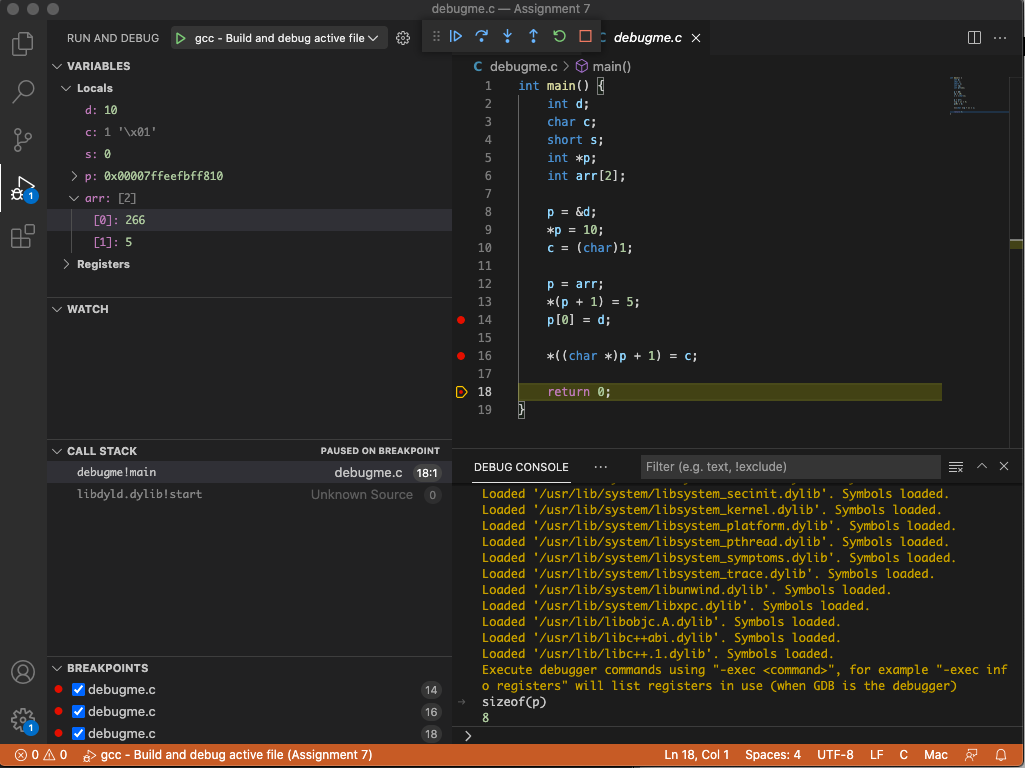
\includegraphics[width=125 mm]{Task1A.png}
			\caption{VS Code window showing the size of variable p using the debug console}
		\end{figure}
		\newpage	
\subsection*{b)}
$\backslash$x01$\backslash$n - this is an indicator of the end of a header and then a new line.
	
		\begin{figure} [h]
			\centering
			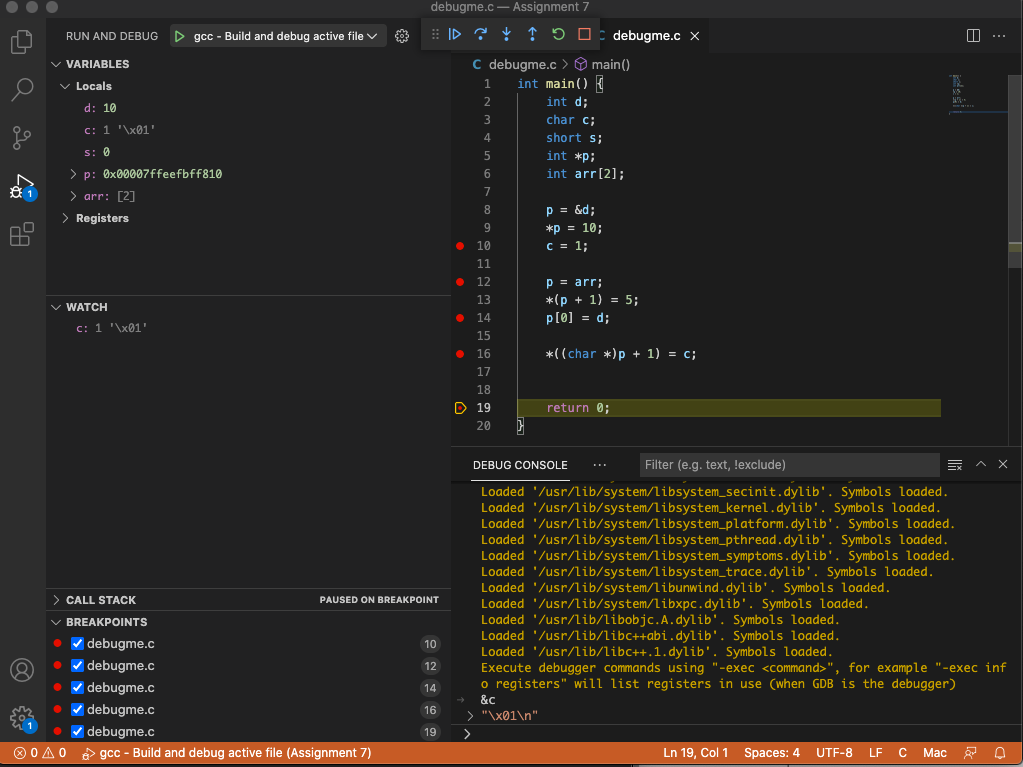
\includegraphics[width=125 mm]{Task1B.png}
			\caption{VS Code window showing the output given for the address of variable c using the debug console}
		\end{figure}
\newpage
\subsection*{c)}
10
		\begin{figure} [h]
			\centering
			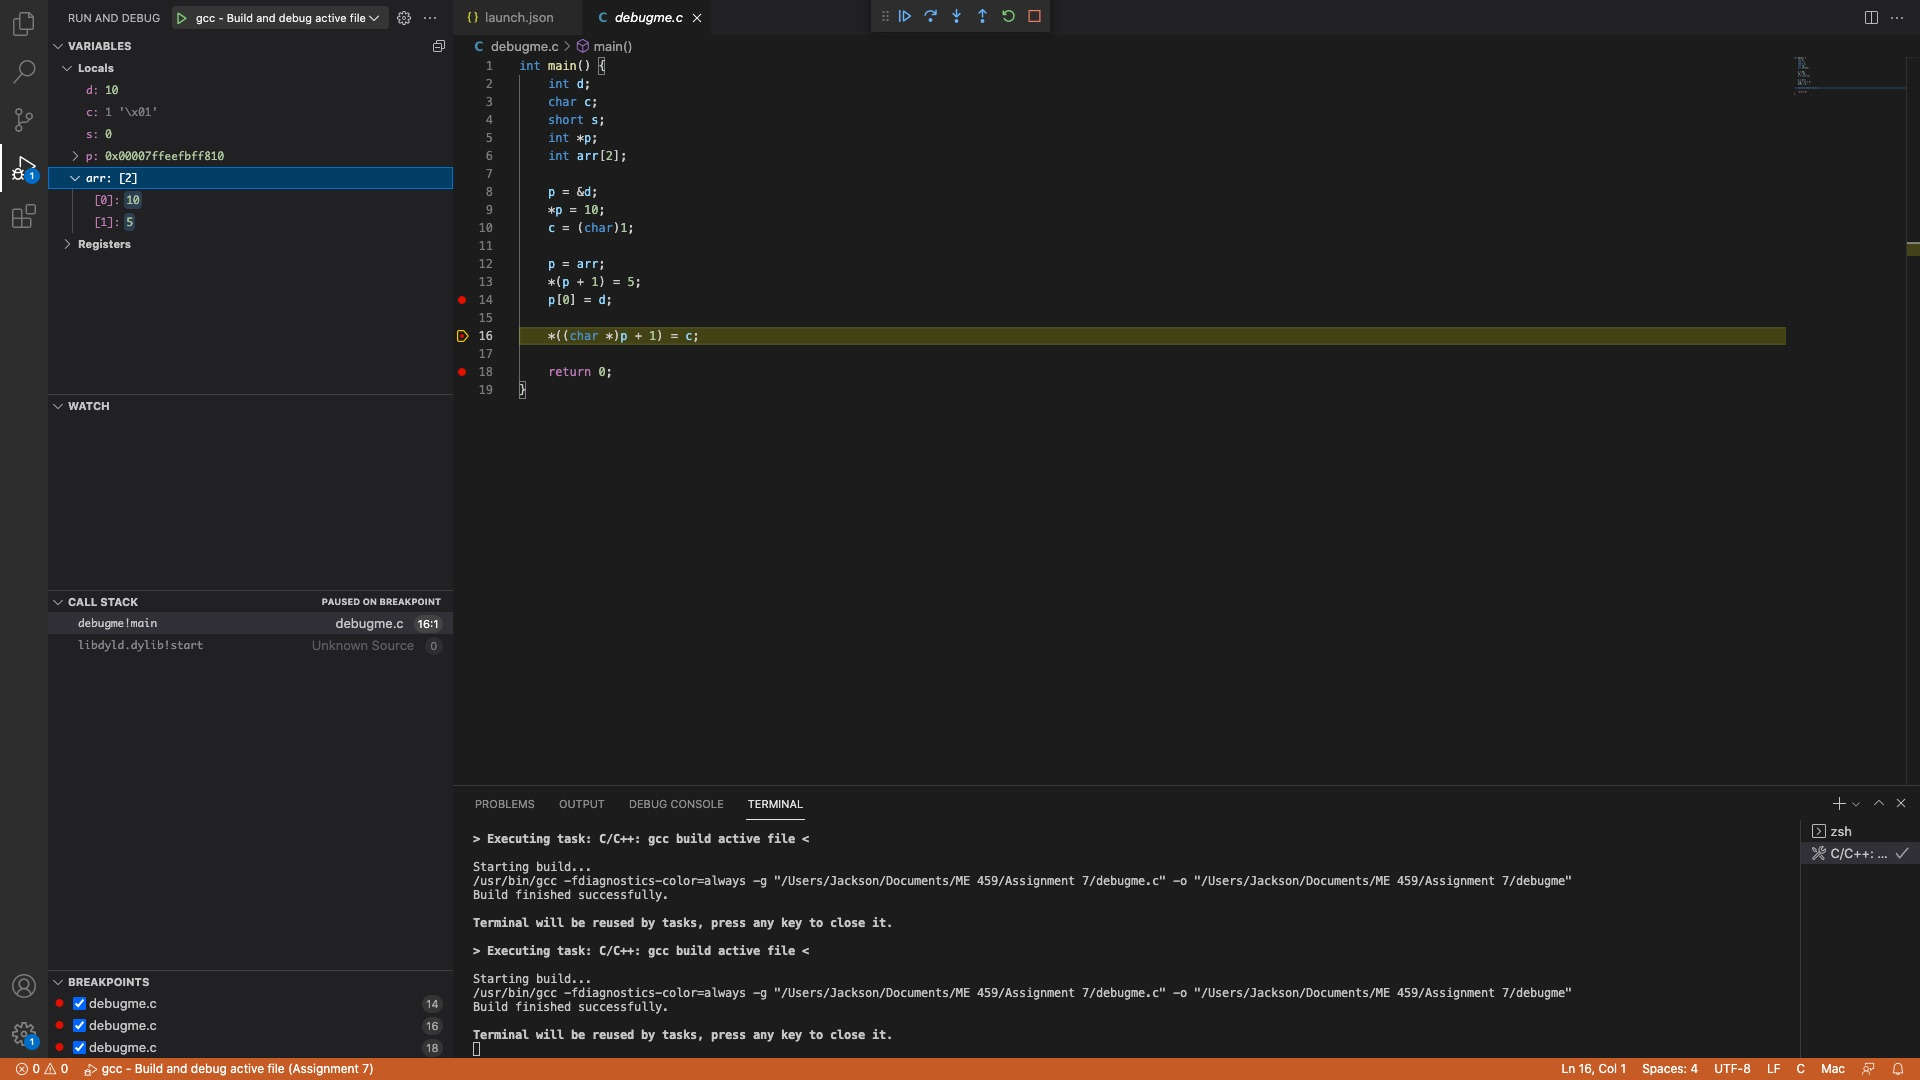
\includegraphics[width=125 mm]{Task1C.jpg}
			\caption{VS Code window showing the value of arr[0] at the requested step of the code}
		\end{figure}
	\newpage	
\subsection*{d)}
266

		\begin{figure} [h]
			\centering
			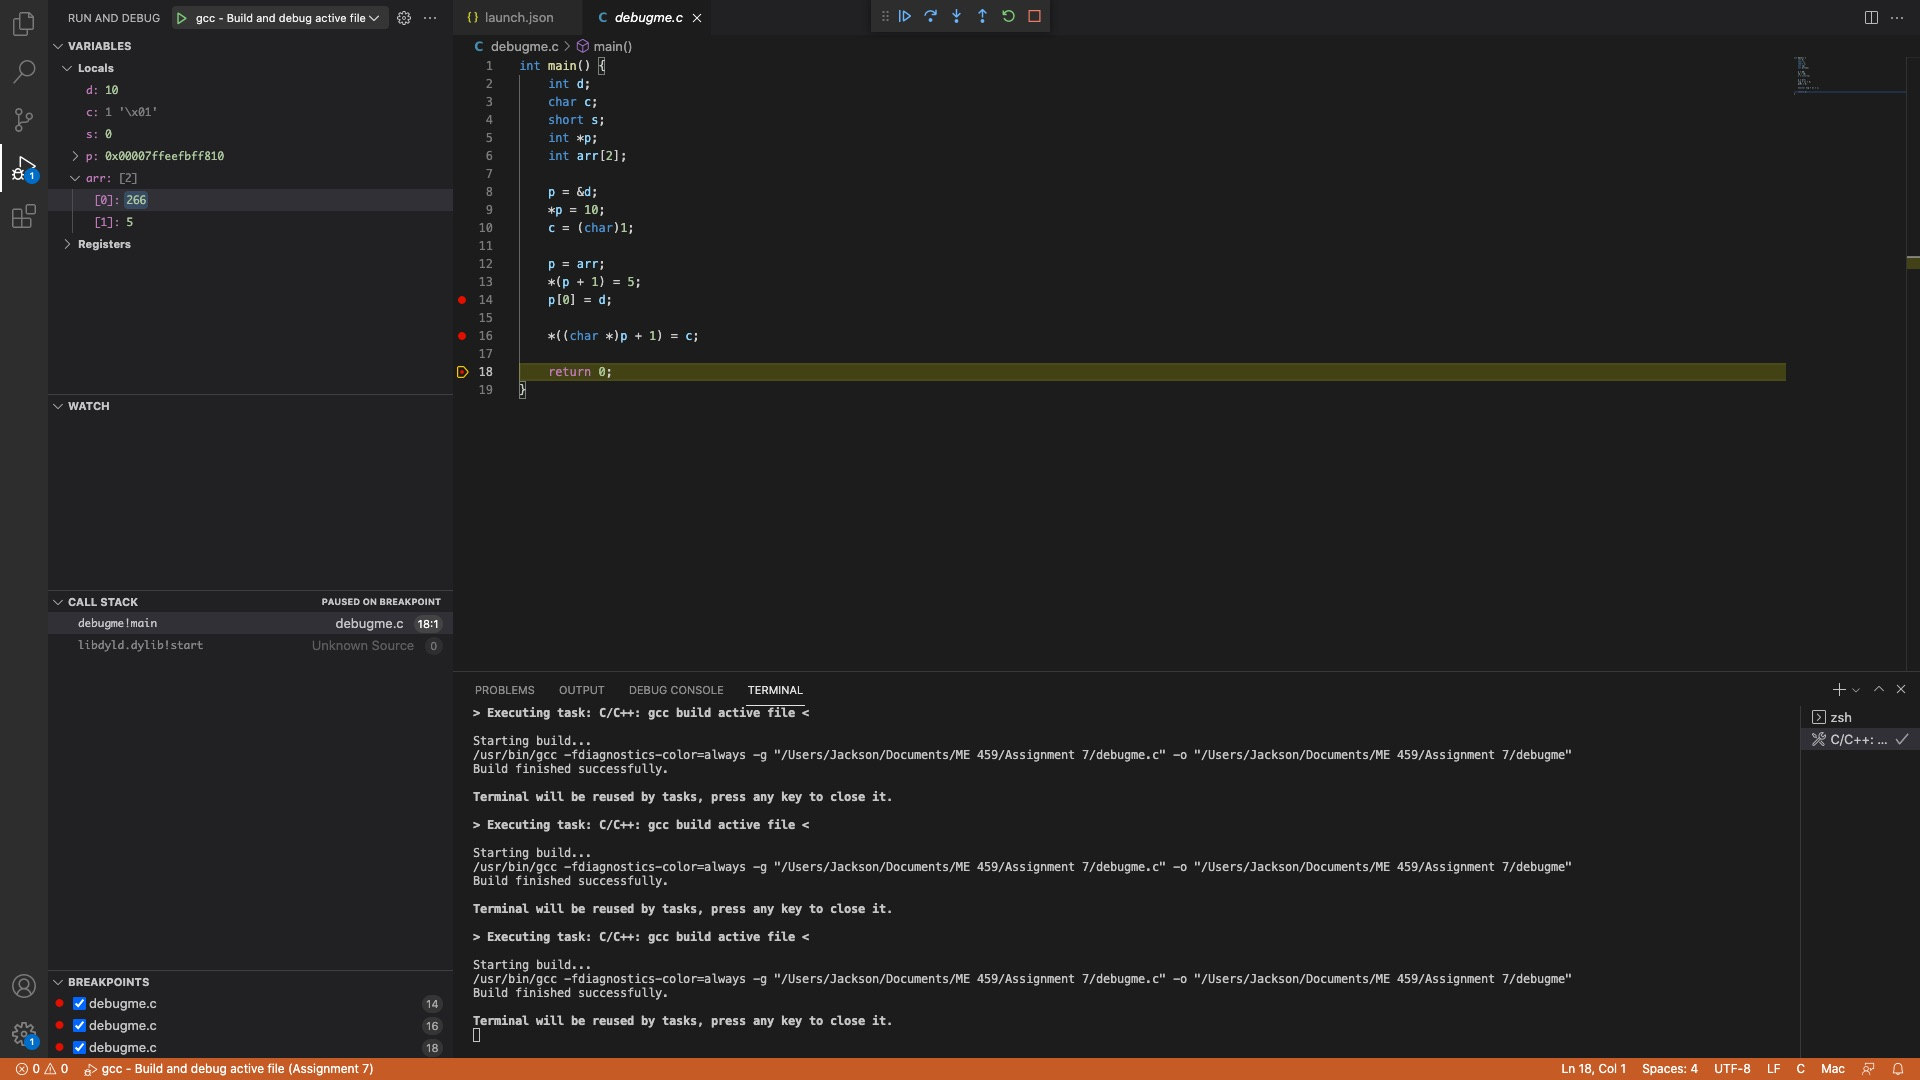
\includegraphics[width=125 mm]{Task1D.jpg}
			\caption{VS Code window showing the value of arr[0] at the requested step of the code}
		\end{figure}
		\newpage	
\subsection*{e)}

The reason that this changes to 266 is that when we cast p to be a char pointer, adding the +1 now moves the pointer to point to the next byte, as chars are only of size 1 Byte.  This is instead of the full 4 byte block which is being read for this location arr[0], as that location is an int.  This then puts a 1 in binary into that byte, which modifies the entire 4 byte read out of the int block within arr.  The modification takes the read out from being 00.....0001010 to 00.......00010001010, which is 266.

		
\end{document}  